%\svnkwsave{$RepoFile: siminos/blog/energy.tex $}
%\svnidlong {$HeadURL$}
%{$LastChangedDate$}
%{$LastChangedRevision$} {$LastChangedBy$}
%\svnid{$Id$}

\chapter{Energy, dissipation, invariant moments}
\label{c-energy}

\renewcommand{\ssp}{x}             % state space point

\ifboyscout
\begin{description}
\item[2008-06-26 PC] moved this to Siminos thesis from
        \texttt{blog/flotsam.tex}.
\item[2009-10-02 PC] moved this back again from
        \texttt{blog/flotsam.tex}.
\item[2012-03-27 PC] In rev.~2294 moved this to
        \texttt{siminos/baroclinic/PCnotes.tex}.
\item[2012-06-06 ES]
Text on invariant moments resurrected from rev. 903. Apparently
disappeared in rev. 904, committed by Predrag. I don't know whether this
excerpt was moved elsewhere. Also I did not try to check whether some
other useful excerpt went MIA in that commit.

\item[2012-06-06 PC] Thanks for amazing detective work! The most
up-to-date version is currently in
\texttt{siminos/baroclinic/PCnotes.tex}, there to persuade Annalisa
and Sebastian to plot some \statesp\ invariants cheaply.

\item[2013-03-31 PC] Annalisa and Sebastian showed no interest, so
the text is back as \texttt{siminos/blog/energy.tex}.

Also search for {\bf 2011-12-06, 2012-02-14 PC} in
\texttt{siminos/lyapunov/blog.tex}.

\end{description}
\fi

\section{\KSe}
\label{s-KS}

\ifboyscout
This section contains material copied from \refref{SCD07}.
\fi

The \KS\ [henceforth KS] system\rf{ku,siv},
which arises in the description of
stability of flame fronts, reaction-diffusion systems and many other
physical settings\rf{KNSks90}, is one of the simplest nonlinear PDEs that
exhibit spatiotemporally chaotic behavior. In the formulation
adopted here, the time evolution of the `flame front velocity'
$u=u(x,t)$ on a periodic domain $u(x,t) = u(x+L,t)$ is given by
\beq
  u_t = F(u) = -{\textstyle\frac{1}{2}}(u^2)_x-u_{xx}-u_{xxxx}
    \,,\qquad   x \in [-L/2,L/2]
    \,.
\ee{ks}
Here $t \geq 0$ is the time, and $x$ is the spatial coordinate.
The subscripts $x$ and $t$ denote partial derivatives with respect to
$x$ and $t$. Spatial periodicity $u(x,t)=u(x+L,t)$
makes it convenient to work in the Fourier space,
\beq
  u(x,t)=\sum_{k=-\infty}^{+\infty} a_k (t) e^{ i k x /\tildeL }
\,,
\ee{eq:ksexp}
with the $1$-dimensional PDE \refeq{ks}
replaced by an infinite set of
ODEs for the complex Fourier coefficients $a_k(t)$:
\beq
\dot{a}_k= \pVeloc_k(a)
     = ( q_k^2 - q_k^4 )\, a_k
    - i \frac{q_k}{2} \sum_{m=-\infty}^{+\infty} a_m a_{k-m}
\,,
\ee{expan}
where $q_k = k/\tildeL$.
Since $u(x,t)$ is real, $a_k=a_{-k}^\ast$, and we can replace the
sum by an $m > 0$ sum.

Due to the hyperviscous damping $u_{xxxx}$, long time solutions of KS
equation are smooth, $a_k$ drop off fast
with $k$.

%%%%%%%%%%%%%%%%%%%%%%%%%%%%%%%%%%%%%%%%%%%%%%%%%%%%%%%%%%%%%%
\begin{figure}[t]
\begin{center}
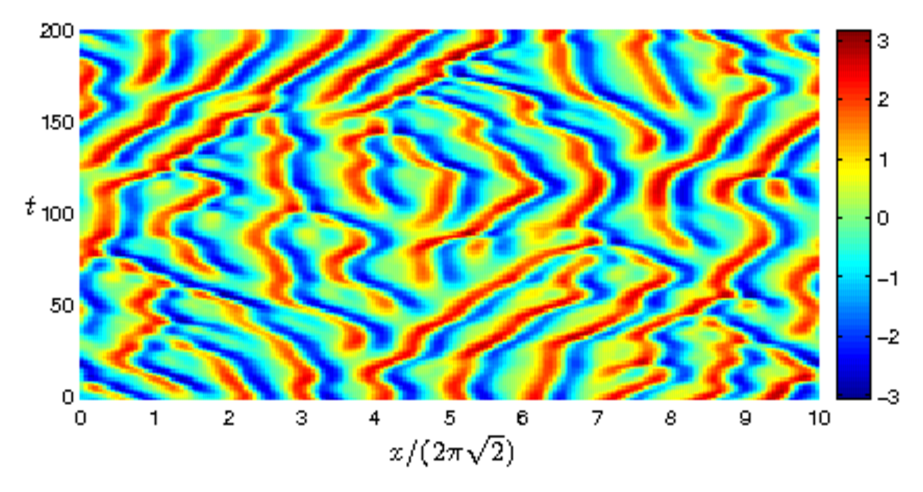
\includegraphics[width=0.9\textwidth]{ks_largeL_cbar_200}
% RLD: longer orbit (to make apperance similar to ks_L22_long_orbit.eps)
% \includegraphics[width=0.9\textwidth]{figs/ks_largeL_cbar.eps}
\end{center}
\caption{
A typical spatiotemporally chaotic solution of the \KSe, system size
$L=20\pi\sqrt{2}\approx 88.86$.  The $x$ coordinate is scaled
with the most unstable wavelength $2\pi\sqrt{2}$, which is
approximately also the mean wavelength of the turbulent flow.
The color bar indicates the color scheme for $u(x,t)$.
     } \label{f:ks_largeL}
\end{figure}
%%%%%%%%%%%%%%%%%%%%%%%%%%%%%%%%%%%%%%%%%%%%%%%%%%%%%%%%%%%%%%%%%%


\section{Energy transfer rates, \KS}
\label{sec:energy}

\ifboyscout
This section contains material copied from \refref{SCD07}.
\fi

In physical settings where the observation times are much
longer than the dynamical `turnover' and Lyapunov times
(statistical mechanics, quantum physics, turbulence) periodic
orbit theory\rf{DasBuch} provides highly accurate predictions
of measurable long-time averages such as the dissipation and
the turbulent drag\rf{GHCW07}. Physical predictions have to
be independent of a particular choice of ODE representation
of the PDE under consideration and
invariant under all symmetries of the dynamics. In this
section we discuss a set of such physical observables for the
1-$d$ KS invariant under reflections and translations. They
offer a representation of dynamics in which the symmetries
are explicitly quotiented out. We shall use these
observables in \refsect{sec:energyL22} in order to
visualize a set of solutions on these coordinates.

The {space average} of a function
$\obser = \obser(\pSpace,t) = \obser(u(x,t))$
on the interval $L$,
\beq
    \expct{\obser} = \Lint{\pSpace}\, \obser(\pSpace,t)
    \,,
    \label{rpo:spac_ave}
\eeq
is in general time dependent.
Its mean value is given by the {time average}
\beq
\timeAver{\obser}
    =
\lim_{t\rightarrow \infty} \frac{1}{t} \int_0^t \! d\tau \, \expct{\obser}
    =
\lim_{t\rightarrow \infty} \frac{1}{t} \int_0^t \!
    \Lint{\tau}  d\pSpace\, \obser(\pSpace,\tau)
    \,.
\label{rpo:tim_ave}
\eeq
The mean value of $\obser = \obser(u_\stagn) \equiv \obser_\stagn$ evaluated on
\eqv\ or {\reqv} $u(\pSpace,t) = u_\stagn(\pSpace-ct)$,
% labeled by  $q$ as in \refeq{reqva},
is
\beq
\timeAver{\obser}_\stagn = \expct{\obser}_\stagn = \obser_\stagn\,.
\label{rpo:u-eqv} \eeq
Evaluation of the infinite time average
\refeq{rpo:tim_ave} on a function of a \po\ or \rpo\
$u_p(\pSpace,t)=u_p(\pSpace+\shift_p,t+\period{p})$ requires only a single
$\period{p}$ traversal,
\beq
  \timeAver{\obser}_p = \frac{1}{\period{p}}
    \int_0^{\period{p}} \! d\tau \, \expct{\obser}
\,.
\label{rpo:u-cyc}
\eeq

Equation \refeq{ks} can be written as
\beq
    u_t=- V_x
        \,,\qquad
    V(x,t)={\textstyle\frac{1}{2}}u^2+u_{x} + u_{xxx}
    \,.
\ee{ksPotent}
If $u$ is `flame-front velocity' then
    \PC{correct using \refref{SCD07}, add ``\expctE, defined in
    refeq{??}''}
can be interpreted as the mean energy
density. So, even though KS is a phenomenological
small-amplitude equation, the time-dependent $L^2$ norm
of $u$,
\beq
    \expctE=
  \Lint{\pSpace}
  V(x,t)=
  \Lint{\pSpace} \frac{u^2}{2}
  \,,
  \label{ksEnergy}
\eeq
has a physical interpretation\rf{ksgreene88} as the average `energy'
density of the flame front. This analogy to the mean kinetic energy
density for the Navier-Stokes motivates what follows.

The energy \refeq{ksEnergy} is intrinsic to the flow,
independent of the particular ODE basis set chosen to
represent the PDE. However, as the Fourier amplitudes are
eigenvectors of the translation operator, in the Fourier
space the energy is a diagonalized quadratic norm,
\beq
\expctE
          =  \sum_{k=-\infty}^{\infty} E_k
\,,\qquad
E_k =
    {\textstyle\frac{1}{2}}|a_k|^2
\,,
\ee{EFourier}
and explicitly invariant term by term
under translations
% \refeq{eq:shiftFour}
and reflections.
% \refeq{KSparity}.

\ifboyscout
Take time derivative of the energy density \refeq{ksEnergy},
substitute \refeq{ks} and integrate by parts. Total derivatives vanish
by the spatial periodicity on the $L$ domain:
\bea
   \dot{\expctE} &=&
     \expct{u_t \, u}
         = - \expct{\left({u^2}/{2} + u_{x} + u_{xxx}\right)_x u }
    \continue
    &=&
\expct{ u_x \, {u^2}/{2} + u_{x}^2 + u_x \, u_{xxx}}
    \,.
\label{rpo:ksErate}
\eea
The first term in \refeq{rpo:ksErate} vanishes by
integration by parts,
\(
3 \expct{ u_x \, u^2}= \expct{(u^3)_x} = 0
\,,
\)
and integrating the third term by parts yet again
one gets\rf{ksgreene88} that the energy variation
\else
\fi
\beq
   \dot{\expctE} = P - D
                \,,\qquad
      P =  \expct{u_{x}^2}
                \,,\quad
      D =  \expct{u_{xx}^2}
\ee{EnRate}
balances the power $P$ pumped in by anti-diffusion $u_{xx}$
against the energy dissipation rate $D$
by hyper-viscosity $u_{xxxx}$
in the KS equation \refeq{ks}.

The time averaged energy density  $\timeAver{E}$
computed on a typical orbit goes to a constant, so
the mean values \refeq{rpo:tim_ave} of drive and dissipation
exactly balance each other:
\beq
    \timeAver{\dot{E}}  =
    \lim_{t\rightarrow \infty}
        \frac{1}{t} \int_0^t d\tau \, \dot{\expctE}
=
      \timeAver{P} - \timeAver{D}
= 0
    \,.
\ee{rpo:EtimAve}
In particular, the \eqva\
and \reqva\ fall onto the diagonal in \reffig{f:drivedrag1}\,(\textit{a}),
and so do time averages computed on \po s and \rpo s:
\beq
\timeAver{E}_p =
\frac{1}{\period{p}} \int_0^\period{p}d\tau \, E(\tau)
    \,,\qquad
\timeAver{P}_p =
\frac{1}{\period{p}} \int_0^\period{p} d\tau \, P(\tau)
    =
      \timeAver{D}_p
    \,.
\label{poE}
\eeq
In the Fourier basis \refeq{EFourier} the conservation of energy on average
takes form
\beq
0 = \sum_{k=-\infty}^{\infty} ( q_k^2 - q_k^4 )\,
    \timeAver{E}_k
\,,\qquad
E_k(t) =  {\textstyle\frac{1}{2}} |a_k(t)|^2
\,.
\ee{EFourier1}
The large $k$ convergence of this series is insensitive to the
system size $L$; $\timeAver{E_k}$ have to decrease much faster than
$q_k^{-4}$.


\subsection{Energy transfer rates for $L=22$ case}
\label{sec:energyL22}

%%%%%%%%%%%%%%%%%%%%%%%%%%%%%%%%%%%%%%%%%%%%%%%%%%%%%%%%%%%%%%%%
\begin{figure}[t]
\begin{center}
 \begin{tabular}{cc}
        ~~~~~~~~(\textit{a})                        &   ~~~~~~~~(\textit{b}) \\
    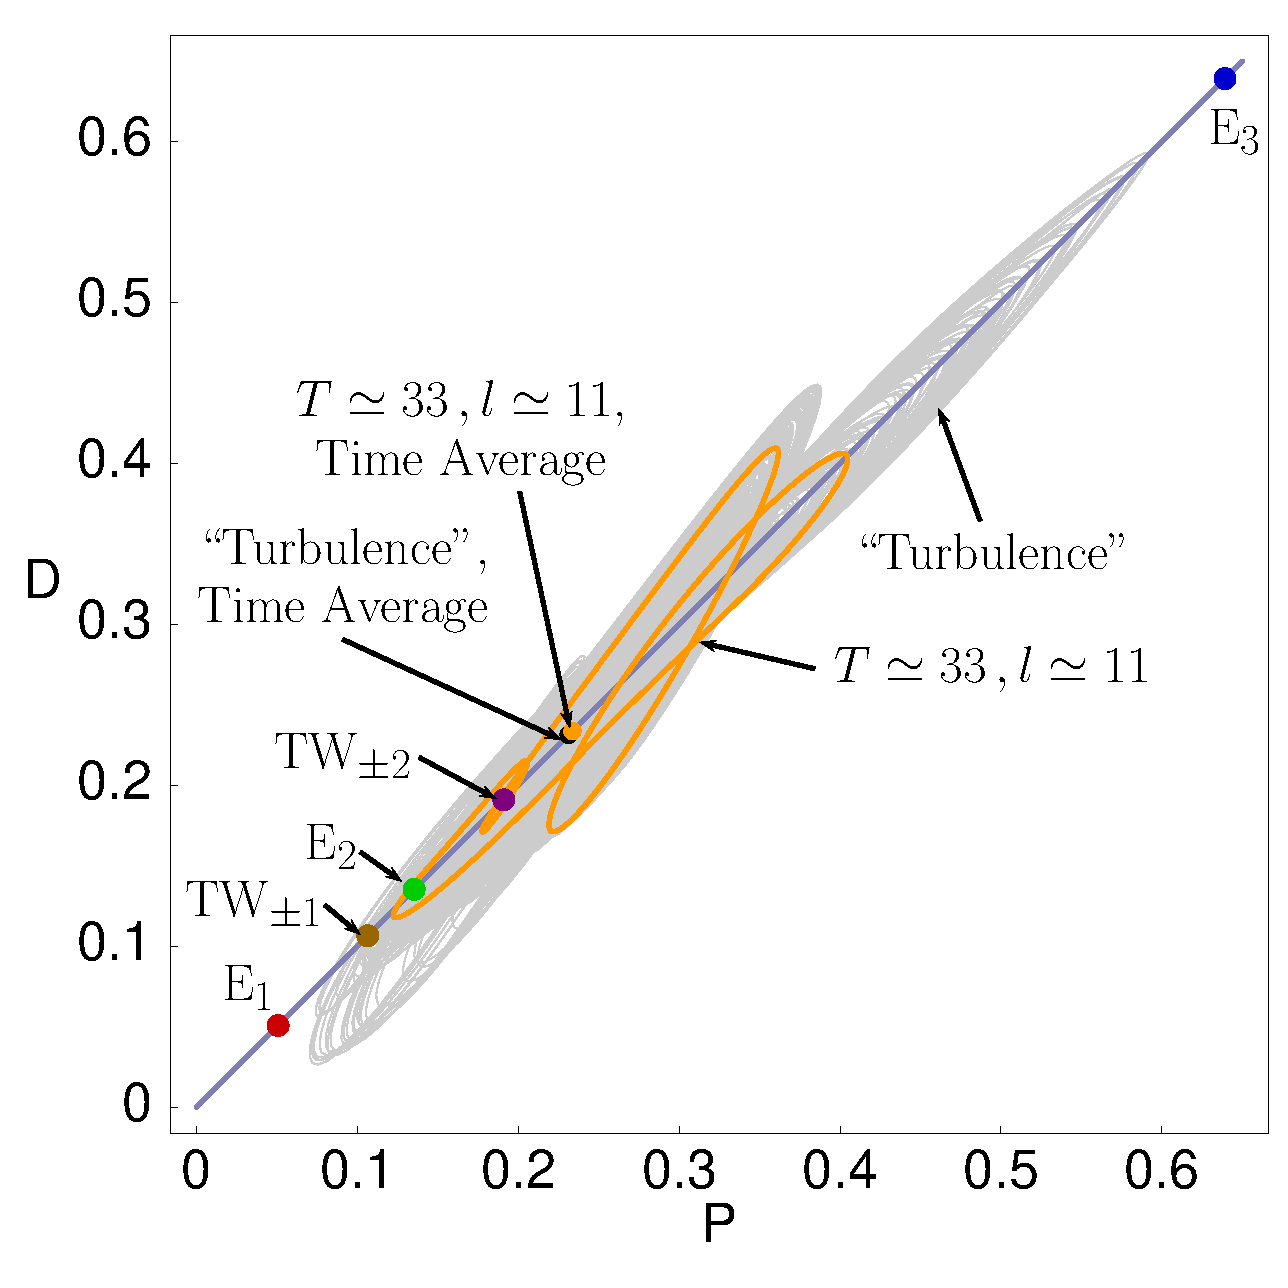
\includegraphics[width=0.46\textwidth, clip=true]{energyBalance_pst}
    & 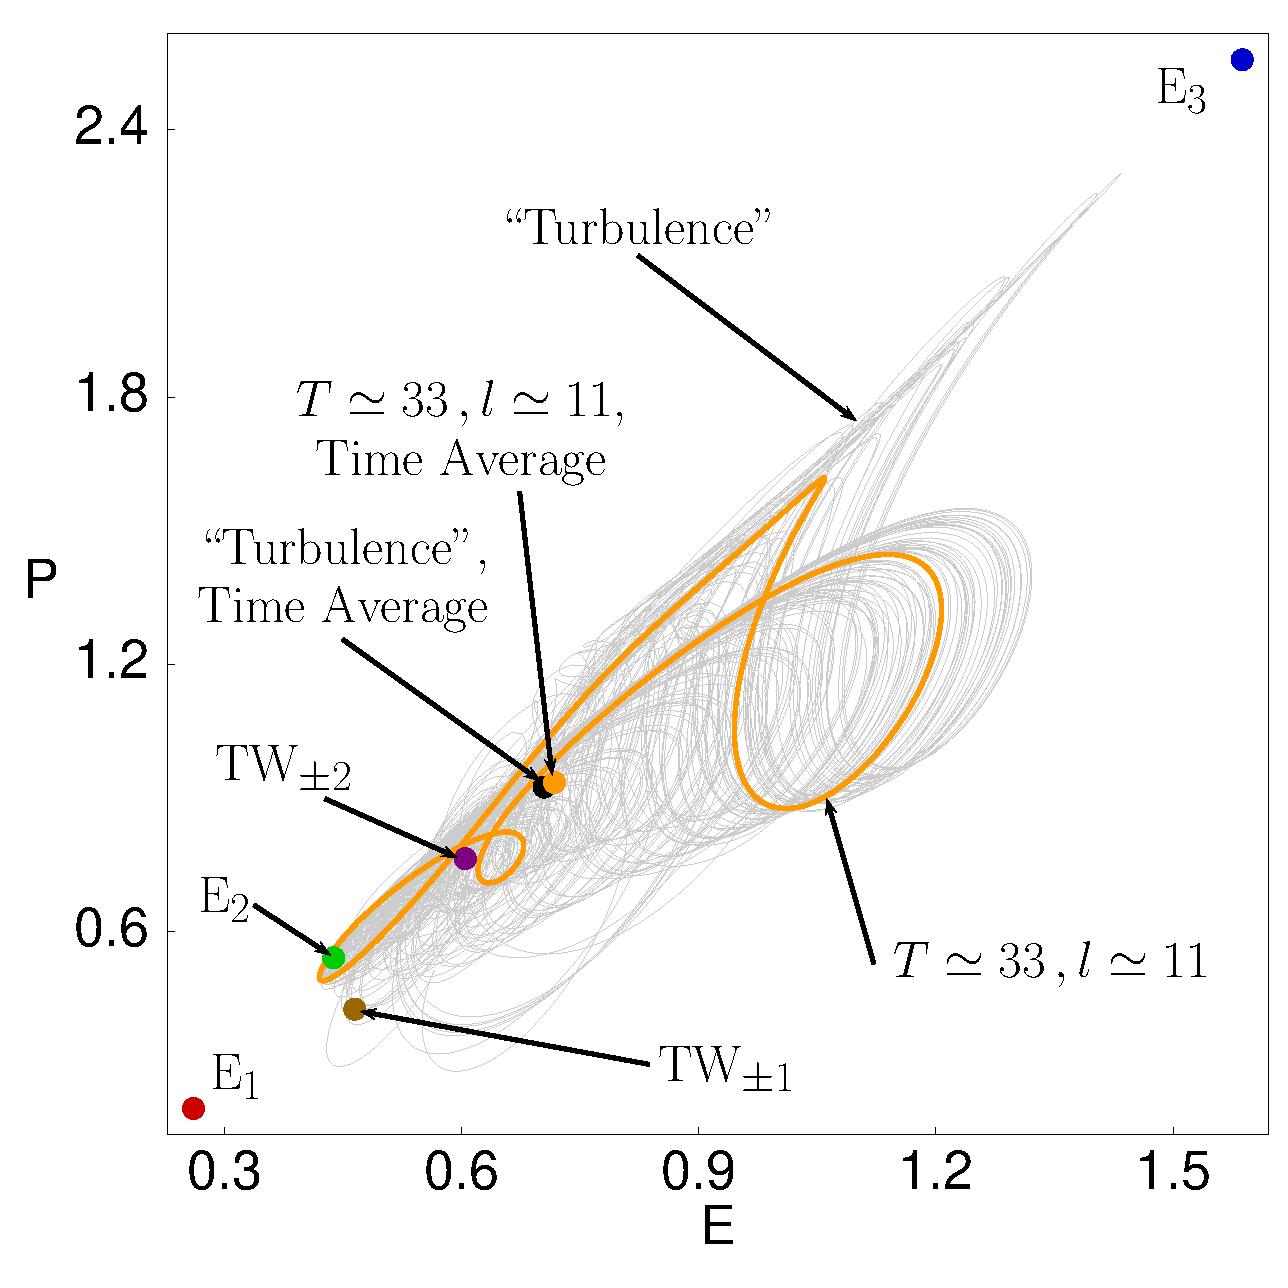
\includegraphics[width=0.46\textwidth, clip=true]{equivaEP_pst}

  \end{tabular}
\end{center}
\caption{
(a) Power input $P$ {\em vs.}
dissipation rate $D$
(b) energy $E$  {\em vs.}
power input $P$,   for several  \eqva\ and \reqva,
a \rpo, and a typical `turbulent' long-time trajectory.
System size $L=22$.
        }
\label{f:drivedrag1}
\end{figure}
%%%%%%%%%%%%%%%%%%%%%%%%%%%%%%%%%%%%%%%%%%%%%%%%%%%%%%%%%%%%%%%%%%

%%%%%%%%%%%%%%%%%%%%%%%%%%%%%%%%%%%%%%%%%%%%%%%%%%%%%%%%%%%%%%%%
\begin{figure}[t]
\begin{center}
 \begin{tabular}{cc}
        ~~~~~~~~(\textit{a})                        &   ~~~~~~~~(\textit{b}) \\
    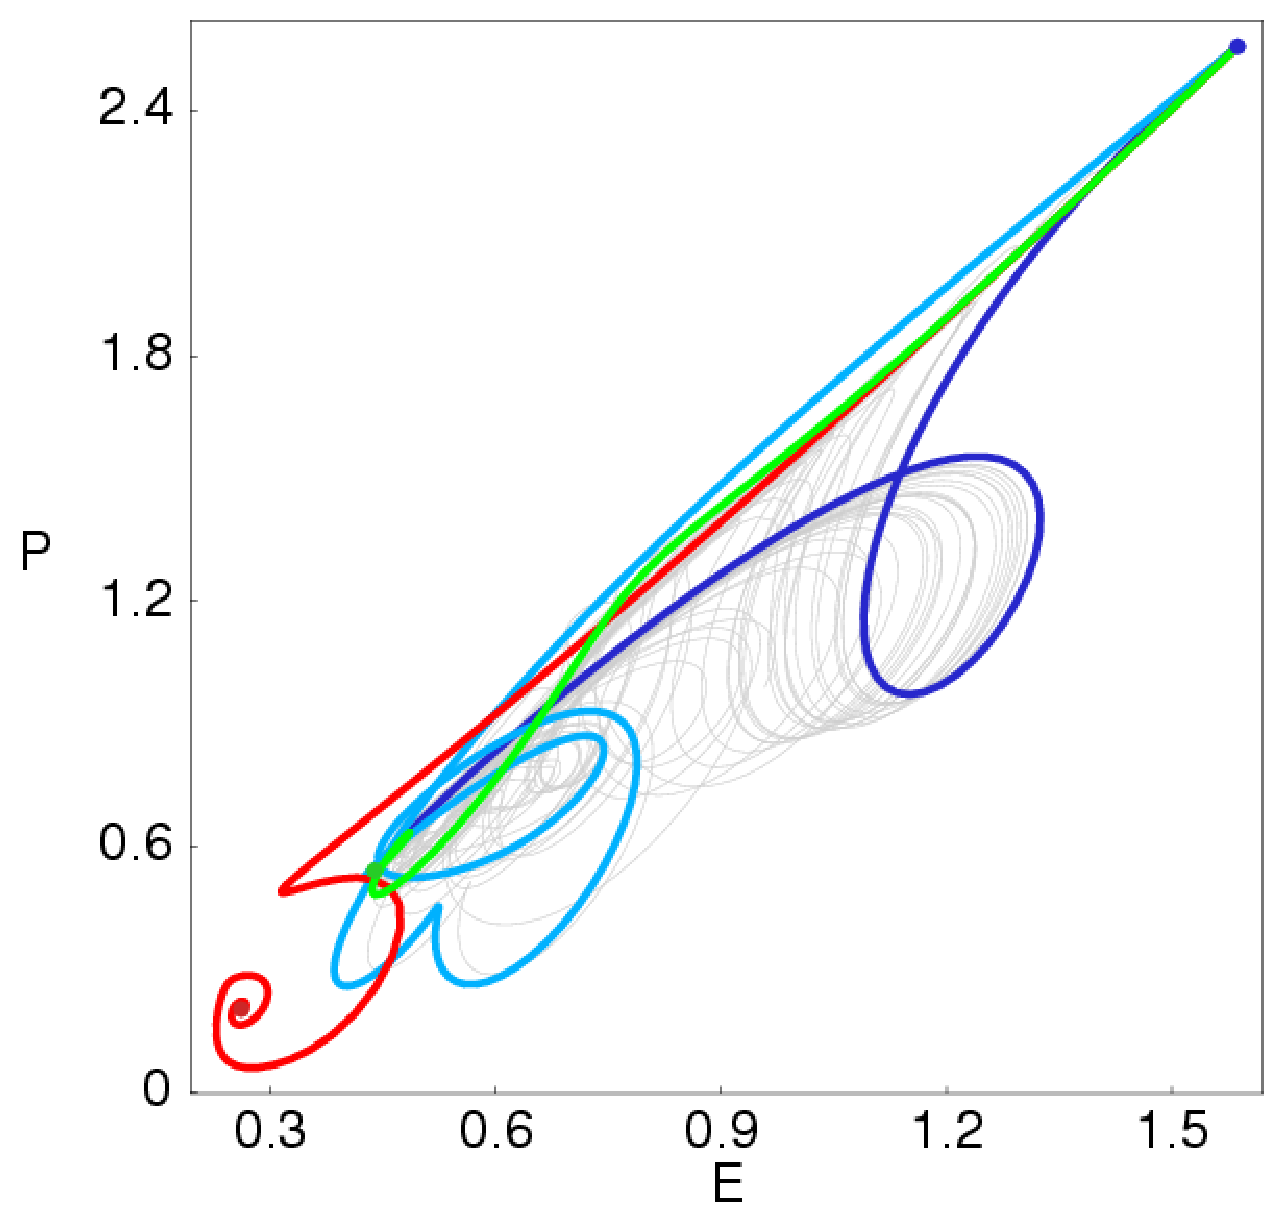
\includegraphics[width=0.46\textwidth, clip=true]{connEP}
     & 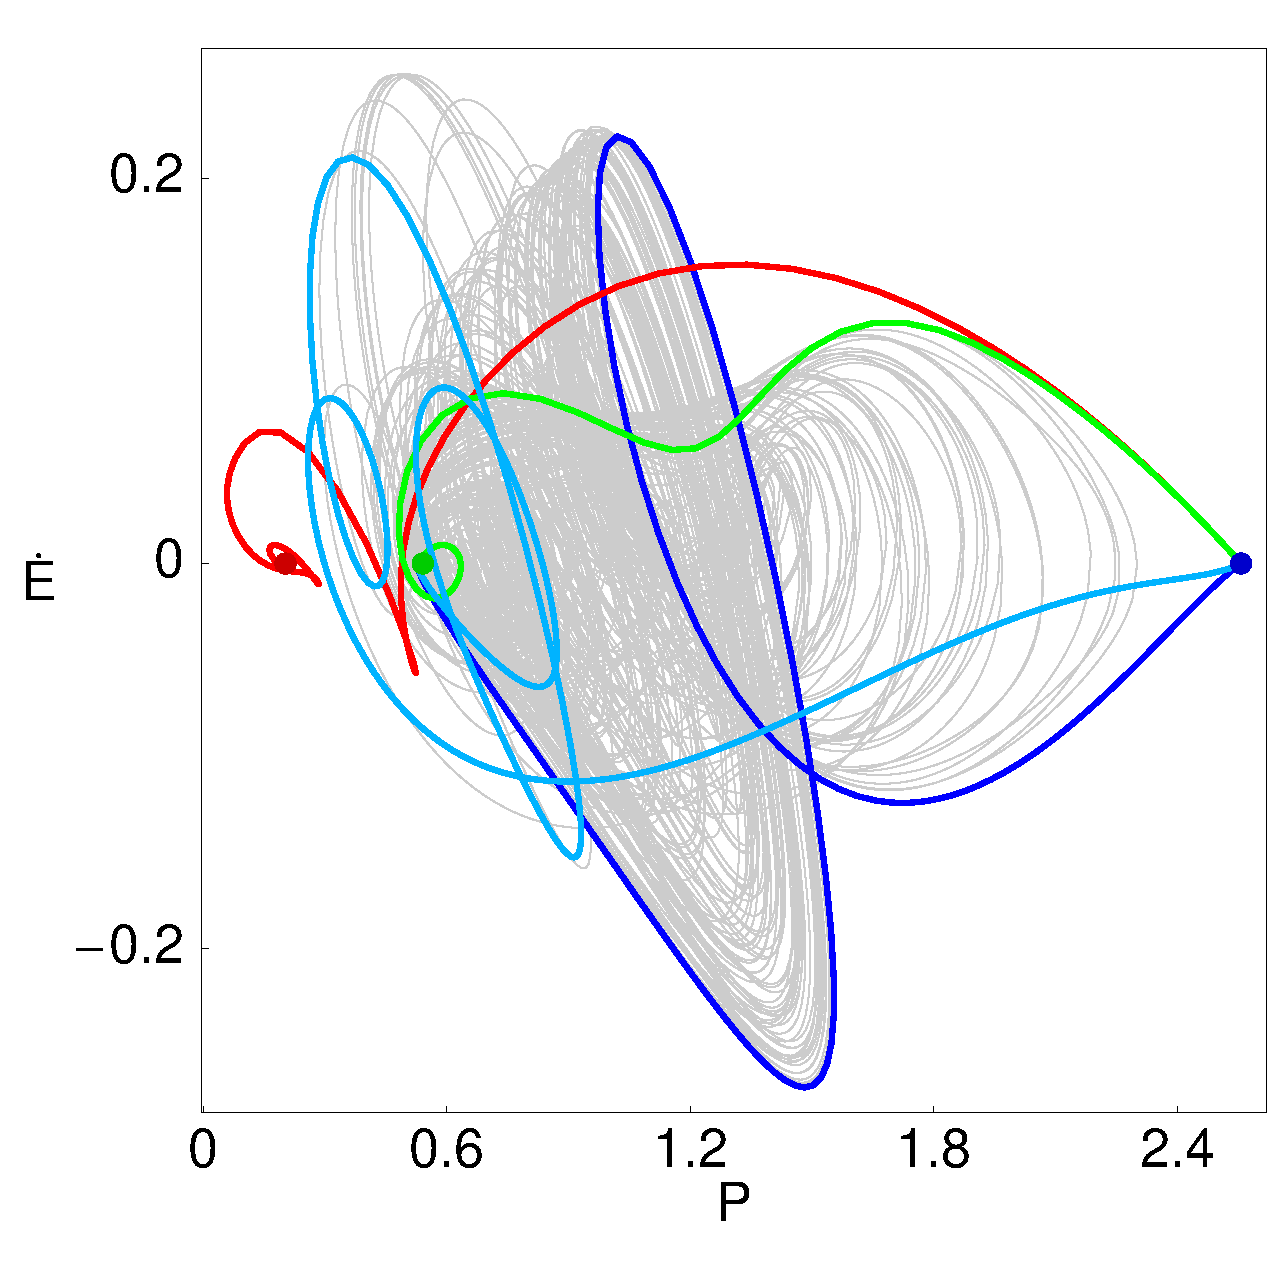
\includegraphics[width=0.46\textwidth, clip=true]{connPEdot}
 \end{tabular}
\end{center}
\caption{
Two projections of the $(E,P,\dot{E})$ representation of the flow.
\EQV{1} (red), \EQV{2} (green), \EQV{3} (blue),
heteroclinic connections from \EQV{2} to $\EQV{3}$ (green),
from $\EQV{1}$ to \EQV{3} (red)
and from \EQV{3} to $\EQV{2}$ (shades of blue), superimposed over
a generic long-time `turbulent' trajectory (grey).
System size $L=22$.
        }
\label{f:drivedragConn}
\end{figure}
%%%%%%%%%%%%%%%%%%%%%%%%%%%%%%%%%%%%%%%%%%%%%%%%%%%%%%%%%%%%%%%%%%

In \reffig{f:drivedrag1} we plot \refeq{EnRate}, the time-dependent
$\dot{\expctE}$ in the power input $P$ {\em vs.}
dissipation rate $D$ plane, for $L=22$ \eqva\ and \reqva,
a selected \rpo, and for a typical `turbulent' long-time
trajectory.

Projections from the $\infty$-dimensional \statesp\ onto the 3-dimensional
$(E,P,D)$ representation of the flow, such as
\reffigs{f:drivedrag1}{f:drivedragConn}, can be misleading.
The most one can say is that if points are clearly separated in an
$(E,P,D)$ plot (for example, in \reffig{f:drivedrag1}
$\EQV{1}$ \eqv\ is outside the recurrent set), they are also separated
in the full \statesp.  Converse is not true -- states of
very different topology can have similar energies.

An example is the \rpo\ $(\period{p},\shift_p) = (32.8,10.96)$
% (see \reffig{f:ks22rpos}(\textit{b}))
which {is the least unstable short \rpo\ we have detected in this system.
It} appears to be well embedded within the turbulent flow. The mean power
$\timeAver{P_p}$ evaluated as in \refeq{poE}, see \reffig{f:drivedrag1},
is numerically quite close to the long-time turbulent time average
$\timeAver{P}$.

\subsection{Further observables, \KS}
\label{sec:moreObs}

\ifboyscout
This section contains some material which has not been included in
publications and/or Siminos and Lan Ph.D. theses.

{\bf PC}: believe it or not, we are now set to compute
    $\timeAver{E}$ and $\timeAver{P}$
    using cycle expansions

Substitution % by \refeq{KSeqvCond}
verifies that for an \eqv\ $\expctE$ is constant:
\[
   \dot{\expctE} =
\expct{ \left({u^2}/{2} + u_{x} + u_{xxx} \right) u_x}
    = \expctE \expct{ u_x }=0
    \,.
\]
\fi


% PC worked out in part with Bridges
An infinite number of identities for moments of
solutions of KS follow\rf{Bridges_priv}. For example,
integrating by parts $\expct{u_{x} u_t}$,
$\expct{u_{xx} u_t}$,
and
$\expct{u^2 u_t}$,
respectively, one obtains \reqva\ relations
\PC{please re-derive these three. Are there more
    important ones that I have missed?
    Also, I - unnecessarily - specialized to \reqva,
    but these identities will be especially useful for \rpo s}
\RLD{I don't quite follow this process of deriving moments.  What is
the reason we look for some combinations of $u$ and its derivatives?
Why not just take $\expct{u_{x\cdots x}}$?
Is there any physical motivation for such combinations,
beyond $E$, $P$ and $D$?  Maybe use things like $\dot{P}$,
$\dot{D}$, etc.?}
\PC{they merit more thought and time than we have now, so let's
   pick them up after the first paper is submitted}
\bea
% \expct{u_{x} u_t}
%     \qquad \to \qquad
c P &=& \expct{u \, u_{x}{}^2}
\label{Bridges1}\\
c P  &=& \expct{u \, u_{xx}{}^2}
\label{Bridges3}
\,.
\eea
\ifboyscout
True for any solution:
\bea
% \expct{u_{xx} u_t}
%     \qquad \to \qquad
\dot{P} &=& 2P - \expct{u_{x}{}^3}  - 2 \expct{u_{xxx}{}^2}
\label{PC1}\\
\dot{D} &=& 2\expct{u_{xxxx}{}^2}
    + 5 \expct{u_{xx}{}^2 u_{x}}  - 2 \expct{u_{xxx}{}^2}
\label{PC2} \\
\ddot{E} &=& \dot{P} - \dot{D} =
     2P - \expct{u_{x}{}^3}
    - 2\expct{u_{xxxx}{}^2} - 5 \expct{u_{xx}{}^2 u_{x}}
\label{PC4}\\
\frac{d}{dt} \expct{u_{x}{}^3} &=&
        3 \expct{u_{x}{}^3u + u_{xx}{}^3}
\label{PC5}
\,.
\eea
\fi
When moments such as \refeq{Bridges1} are added as
coordinate axes to \reffig{f:drivedragConn}, \reqva\ and
\rpo s are separated from \eqva\ and \po s. Furthermore,
as higher moments have more and more powers of $u$ and derivatives
$u_{xx\cdots x}$, their magnitudes should be strongly suppressed,
providing a symmetry-invariant basis set that can be safely truncated to
a finite-dimensional \statesp.

For example, the energy of \reqva\ \REQV{\pm}{2} which
seems close to the
mean turbulent energy in \reffig{f:drivedrag1} is separated
from it when plotted along the
$\expct{u \, u_{x}{}^2}$ moment, where according to
\refeq{Bridges1} it takes nonzero value $c P$.

%%%%%%%%%%%%%%%%%%%%%%%%%%%%%%%%%%%%%%%%%%%%%%%%%%%%%%%%%%%%%%%%%%%%%%%%%%
\ifboyscout\else\newpage\fi

\exercise{\KS\ energy transfer rates.}{ \label{exer:KSenergy}
% Predrag                           1apr2013
\index{energy!Kuramoto-Sivashinsky}
\index{dissipation! rate, Kuramoto-Sivashinsky}
    %
\PC{ChaosBook: add this to Problems/exerPDEs}
\begin{itemize}
\item[(a)]              \Points{2}
    Derive \refeq{ksEnergy} from \refeq{ksPotent}.
\item[(b)]              \Points{2}
    Derive \refeq{EnRate}.
\item[(c)]              \Points{2}
    Prove that for an \eqv\ $\expctE$ is constant:
\item[(d)]              \Points{6 bonus}
    Derive formulas for
    $\dot{P}$, $\dot{D}$, $\ddot{E}$
    and $\frac{d}{dt} \expct{u_{x}{}^3}$
    in terms of space averages $\expct{\cdots}$.
\item[(e)]              \Points{4 bonus for all}
    Invent another such formula.
\end{itemize}

        }% end \exercise{\KS\ energy transfer rates

\exercise{\NS\ energy transfer rates.}{ \label{exer:NSenergy}
% Predrag                           1apr2013
\index{energy!Navier-Stokes}
\index{dissipation! rate, Navier-Stokes}
    %
\PC{ChaosBook: add this to Problems/exerPDEs}
\HREF{http://www.claymath.org/millennium/Navier-Stokes_Equations/}
{The Millenium Prize} wants you to ponder the \NSe\
\beq
\pde_t v_i + v_j\pde_j v_i = - \pde_i p + \nu \pde_{jj} v_i
\ee{FrischNS}
in a periodic 3$D$ box
of size $[L\times L\times L]$.
The {space average} of a function
$\obser = \obser(\pSpace,\zeit) = \obser(v(\pSpace,\zeit))$
on the interval $L$ is given by
\beq
    \expct{\obser} =
    \frac{1}{L^3}\!\oint d\pSpace^3 \obser(\pSpace,\zeit)
    \,,
\,.
\ee{FrischAver}

\begin{itemize}
\item[(a)]               \Points{2}
    Prove conservation of momentum
\beq
\frac{d~}{dt} \expct{v_i} = 0
\ee{FrischConvMom}
\item[(b)]              \Points{4}
    Prove power-dissipation rate relation
\beq
\frac{1}{2}\frac{d~}{dt} \expct{v^2} = - \nu \expct{|\omega^2|}
\ee{FrischConvMom}
\item[(c)]              \Points{4 bonus}
    Prove conservation of helicity.
\beq
\frac{1}{2} \frac{d~}{dt} \expct{v\cdot\omega}
= - \nu \expct{\omega\cdot\nabla\times\omega}
\ee{FrischHelic}
\item[(d)]             \Points{6 bonus for all}
    While you are on the roll: derive another such formula. Pipe or
    \pCf\ power-dissipation relation $\dot{E}=P -{D}$ would be
    particularly useful.
\end{itemize}

        }% end \exercise{\KS\ energy transfer rates

\exercise{Channelflow.org.}{ \label{exer:channelflow}
% Predrag                           1apr2013
(Bonus) Please download the code.
\HREF{http://channelflow.org/dokuwiki/doku.php?id=docs:tutorial}{Tutorial}
and
\HREF{http://channelflow.org/dokuwiki/doku.php?id=gtspring2009:howto}
{HowTo}
might be helpful.
        }% end \exercise{\KS\ energy transfer rates


\ifboyscout\else\newpage\fi

\solution{exer:KSenergy}{\KS\ energy transfer rates.}{
\begin{itemize}
  \item[(a)]
Integrate by parts, use periodicity.
  \item[(b)]
Take time derivative of the energy density \refeq{ksEnergy},
substitute \refeq{ks} and integrate by parts. Total derivatives vanish
by the spatial periodicity on the $L$ domain:
\bea
   \dot{\expctE} &=&
     \expct{u_t \, u}
         = - \expct{\left({u^2}/{2} + u_{x} + u_{xxx}\right)_x u }
    \continue
    &=&
\expct{ u_x \, {u^2}/{2} + u_{x}^2 + u_x \, u_{xxx}}
    \,.
\label{rpo:ksErate}
\eea
The first term in \refeq{rpo:ksErate} vanishes by
integration by parts,
\(
3 \expct{ u_x \, u^2}= \expct{(u^3)_x} = 0
\,,
\)
and integrating the third term by parts yet again
one gets \refeq{EnRate}.
  \item[(c)]
This verifies that for an \eqv\ $\expctE$ is constant:
\beq
   \dot{\expctE} =
\expct{ \left({u^2}/{2} + u_{x} + u_{xxx} \right) u_x}
    = \expctE \expct{ u_x }=0
    \,.
\ee{exer:PC3}
  \item[(d)]
\bea
% \expct{u_{xx} u_t}
%     \qquad \to \qquad
\dot{P} &=& 2P - \expct{u_{x}{}^3}  - 2 \expct{u_{xxx}{}^2}
\label{exer:PC1}\\
\dot{D} &=& 2\expct{u_{xxxx}{}^2}
    + 5 \expct{u_{xx}{}^2 u_{x}}  - 2 \expct{u_{xxx}{}^2}
\label{exer:PC2} \\
\ddot{E} &=& \dot{P} - \dot{D} =
     2P - \expct{u_{x}{}^3}
    - 2\expct{u_{xxxx}{}^2} - 5 \expct{u_{xx}{}^2 u_{x}}
\label{exer:PC4}\\
\frac{d}{dt} \expct{u_{x}{}^3} &=&
        3 \expct{u_{x}{}^3u + u_{xx}{}^3}
\label{exer:PC5}
\,.
\eea
  \item[(e)] $\cdots$
\end{itemize}
    } %end \solution{\KS\ energy transfer rates

\solution{exer:NSenergy}{\NS\ energy transfer rates.}{
% Predrag                           1apr2013
    %
\PC{ChaosBook: add this to Problems/exerPDEs}
See Uriel Frisch\rf{frisch}, p.~19.

        }% end \solution{\KS\ energy transfer rates

\renewcommand{\ssp}{a}             % state space point
